%!TeX root = ../index.tex

\section{Introduction}\label{sec:introduction}

\section{Reactive \acrlongpl{is}}

\citeauthor{boner_reactive_2014} describe how modern \glspl{is} of different domains all exhibit similar qualities.
\citetitle{boner_reactive_2014} summarizes those qualities and dubs the systems which feature them \enquote{reactive} \parencite{boner_reactive_2014}.
Put into the context of the quality dimensions defined by the \citetitle{iso_25010_2011} standard,
the reactive qualities cover only \enquote{Performance Efficiency} and \enquote{Reliability}.
While the other quality dimensions of the \citeauthor{iso_25010_2011} standard are certainly also important, this work focuses on the two mentioned before.\todo{improve sentence flow}

To quickly summarize \cite{boner_reactive_2014}, reactive systems are:

\begin{description}
  \item[Responsive] The system has low upper ceilings for its response times and meets these consistently.
  \item[Resilient] The system remains responsive in the face of failure.
  \item[Elastic] The system remains responsive under varying workload.
\end{description}

All of these qualities cover the technological perspective on reactive systems.
However, there is a business perspective to the term, too.
Reactive systems also need to be flexible.
They need be able to to respond and change quickly according to changing requirements.
For example due to changing customer or market needs.
\citeauthor{beck2001agile} describe this quality as part of their \citetitle{beck2001agile} \parencite{beck2001agile}.
This work will refer to this quality as \emph{flexibility} from here on.

Different design and work patterns have emerged to create reactive systems.
One that is increasingly popular is microservice architecture \parencite{loukides_microservice_adoption_2020}.

\subsection{Microservice Architecture}

\citeauthor{richardson_microservices_2019} defines the microservice pattern as \enquote{an architectural style that functionally decomposes an application into a set of services} \parencite[11]{richardson_microservices_2019}.
The services are supposed to be loosely coupled, independently deployable, and scalable.
They are also small enough to be developed by a single, largely autonomous team.
The compartmentalization of the application also allows for it to tolerate partial failure.
If a single service fails, the rest of the application may stay partially functional.
\parencite[14f.]{richardson_microservices_2019}
These qualities contribute to the application's overall elasticity, resilience, and flexibility.

It is pointed out by \citeauthor{fowler_microservices_2014} that microservices commonly integrate with each other via synchronous communication protocols like \glspl{rpc} or HTTP \parencite{fowler_microservices_2014}.
This introduces different forms of coupling to the system.
First, the services need to know routes via which they can reach another directly.
Second, the services need to know not only the structure of the data they exchange but also each others' \gls{api}.
Last, the synchronous nature of the communication couples the services in the dimension of time.
A service either completes a request in time, or the request reaches a timeout.
It is for this reason that many applications rely on asynchronous, message-driven communication via \gls{mom} \parencite{fowler_microservices_2014}.

\subsection{\acrlong{mom}}

\cite{boner_reactive_2014} defines one additional quality of reactive systems: message-driven.
Message-driven systems \enquote{rely on asynchronous message-passing to
establish a boundary between components that ensures loose coupling, isolation,
location transparency, and provides the means to delegate errors as messages.} \parencite{boner_reactive_2014}
As shown in figure \ref{fig:reactive-traits}, the message-driven quality forms the foundation for achieving all other qualities of a reactive system.

\begin{figure}
  \centering
  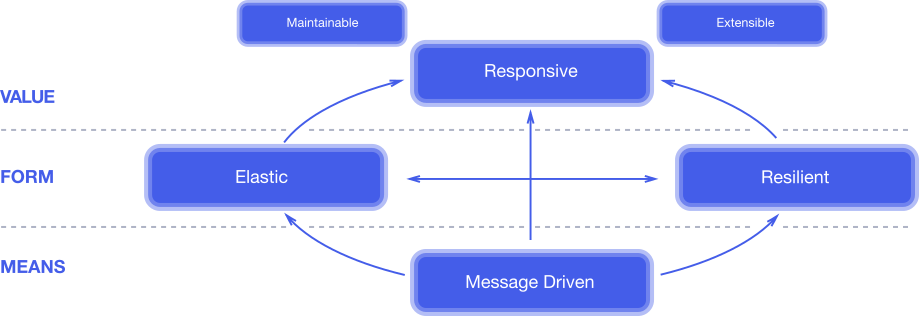
\includegraphics[width=\linewidth]{reactive-traits.png}
  \caption{The Qualities of a Reactive System \parencite{boner_reactive_2014}}
  \label{fig:reactive-traits}
\end{figure}

\cite{banavar_case_1999} coined the term of \acrlong{mom} for dedicated software components meant to integrate disparate applications in a distributed system by facilitating asynchronous message-passing between them.
\citeauthor{banavar_case_1999} based their work in part on the publish/subscribe semantics described in \cite{oki_information_1993} which are still present in the more comprehensive exploration of \gls{mom} in \cite{curry_message-oriented_2004} and prevail to this day.

There exist multiple established protocols which implement the patterns of \gls{mom} like AMQP and MQTT \parencites{amqp}{mqtt} and software solutions implementing the protocols (also called message brokers) like RabbitMQ or Mosquitto \parencites{rabbitmq}{mosquitto}.
While implementation details and terminology might vary between protocols and brokers, the general patterns are the same.

Clients \emph{publish} packets of data called \emph{messages} to a logical communication channel managed by the broker.
From here on, the text refers to such communication channels as \emph{topics}.
Clients can also \emph{subscribe} themselves to these topics and receive messages published to them.
Message delivery may be transient or persistent, meaning that messages are either delivered immediately to the subscribers of a topic by the broker or that the broker stores the messages in subscriber-specific, first-in-first-out queues.
Queues allow subscribers to consume messages at their own pace and become temporarily unavailable without losing messages.
\parencite{curry_message-oriented_2004}

However, one popular message broker does things a little differently.
The following section examines the ways in which Apache Kafka implements the patterns of \gls{mom}.

\subsection{Apache Kafka}

The LinkedIn employees \citeauthor{kreps_kafka_2011} introduced their new \enquote{Event Streaming Platform} \emph{Kafka} in \citeyear{kreps_kafka_2011} \parencite{kreps_kafka_2011}.
Over a decade later, the project has since joined the Apache foundation and \enquote{[m]ore than 80\% of all Fortune 100 companies trust, and use [it]} \parencite{apache_software_foundation_apache_nodate}.

\citeauthor{kreps_kafka_2011} describe Kafka as \enquote{[\ldots] a novel messaging system for log processing [\ldots] that combines the benefits of traditional log aggregators and messaging systems.} \parencite{kreps_kafka_2011}.
Similar to traditional \gls{mom}, \emph{producers} publish messages to logical communication channels called topics and \emph{consumers} can subscribe to topics to consume messages.
In contrast to traditional \gls{mom} however, topics are backed by one or more \emph{partitions}, an append-only data structure stored on the hard drive of a server running Kafka called a \emph{broker}.
Therefore, Kafka persists all messages sequentially for a configurable time even if the brokers restart.
Producers address messages to a topic but actually always publish them to a partition.
To which partition they publish a message if there are multiple is determined by a partitioning algorithm.
Partitions can also have replicas on other brokers, making Kafka tolerant against the failure of single servers.
\parencite{kreps_kafka_2011}

A message in Kafka does not have a dedicated ID.
Instead, a message's logical offset within its partition identifies it.
Consumers consume messages sequentially and move a pointer to the next offset after they have processed the message at the current position.
Furthermore, consumers can form groups in which no two members subscribe to the same partition, thereby achieving a simple load balancing mechanism.
That also makes the number of partitions that a topic has the maximum degree of parallelism with which consumers can consume its messages.
\parencite{kreps_kafka_2011}

Kafka is not only useful for processing the kinds of log data that are proposed by \citeauthor{kreps_kafka_2011}: activity (e.~g. user logins, clicks, \enquote{likes}, \ldots) and operational data (e.~g. \gls{cpu} or disk utilization, HTTP requests, \ldots) \parencite{kreps_kafka_2011}.
\citeauthor{stopford_designing_2018}, for example, outlines how Kafka can serve as the basis of a business application's entire state management and internal communication.
His design implements concepts from the \gls{ddd} community like Event Sourcing \parencite{fowler_event_sourcing_2005} and \gls{cqrs} \parencite{fowler_cqrs_2011} with Kafka's log-based messaging at the center \parencite{stopford_designing_2018}.
The potential use cases of Kafka are therefore plentiful.

\section{Schemas}

This section examines schema technologies and how they can be used to make a distributed \gls{is} more reactive.
For the latter purpose, the text proposes a hypothetical design of an \gls{is} using microservices and Kafka as a \gls{mom}.
This example serves as a basis to analyze what advantages the introduction of Apache Avro as a schema technology provides, what new problems it causes and how to address them.\todo{reason for choosing avro/kafka}

Schemas are structured documents that describe the structure of other documents.
Schema technologies like XML schema, JSON schema, Apache Avro, or Google's Protocol Buffers (ProtoBuf) focus on describing the \emph{syntactical} structure of a document while others like the \gls{owl} or the \gls{rdf} intend to also define the \emph{semantic} structure of documents as well \parencites{xmlschema}{jsonschema}{avro}{protobuf}{owl}{rdf}.
Furthermore, some technologies like Avro or ProtoBuf do offer other capabilities beyond describing the structure of documents, like describing the structure of \gls{rpc}-based \glspl{api} \parencites{avro}{protobuf}.

% \subsection{Apache Avro}

% Apache Avro is a schema technology for describing the syntactical structure of documents and \gls{rpc}-based \glspl{api}.
Beyond the schema definitions, Avro also provides a compact binary serialization format and support for schema evolution.
Listing \ref{lst:avro-schema-person} shows an example for an Avro schema describing a customer entity.
\parencite{avro}


\begin{listing}[H]
  \inputminted{json}{assets/src/Customer.avsc}
  \caption{Simplified Avro Schema of a Customer Entity}\label{lst:avro-schema-person}
\end{listing}

When a client uses Avro's tooling to serialize a document to binary, Avro expects the document's schema as an input beside the actual data.
The schema is used to write the serialized data sequentially without any type information. 
This makes the resulting byte stream compact but also hard to de-serialize without the document's schema.
The schema with which a document was serialized is called the \emph{writer} schema.
\parencite{avro}

A client that uses Avro to de-serialize a byte stream into a document might expect a certain structure for the document.
That is called the \emph{reader} schema.
Avro expects both the writer and the reader schema as inputs besides the serialized byte stream to de-serialize a document.
\parencite{avro}

In many cases, the writer and reader schema may be equal, yet in some, they might be different.
For example, if an application uses Avro to serialize data to the hard drive and changes its data model and schemas in the meantime.
When the application later reads the data and attempts to de-serialize it, it can use the changed schema as the reader schema but must use the old schema as the writer schema.
Only in this way is Avro able to properly read the serialized data.
If the differences between the schemas are \emph{compatible} Avro can map the data from the reader to the writer schema and successfully de-serialize the data.
If not, then the de-serialization fails.
\parencite{avro}

In this way, Avro supports the compatible evolution of schemas.
Compatible changes are, for example, the adding of a new field with a default value or the removal of a field with a default value.
With Avro's support for field name aliases, fields can even be renamed in a compatible manner.
The Avro project also includes tooling to check the compatibility of two schemas.
\parencite{avro}

% \citeauthor{kreps_kafka_2011} chose Apache Avro as the serialization protocol for their message payloads due to its efficiency and schema evolution capabilities \parencite{kreps_kafka_2011}. 

\section{Schemas in Reactive \acrlongpl{is}}

To examine how schemas can fit into a reactive system, consider the following example:
A web-shop application where users can view the current catalog of products and place orders.
The example omits other aspects of a web-shop for simplicity.
The web-shop's architecture follows the microservice architecture and uses Kafka as a \gls{mom} to be reactive.

\subsection{A Reactive Web-Shop Application}

Figure \ref{fig:web-shop} presents a simple overview of the shop's components and their communication.

\begin{figure}[H]
  \centering
  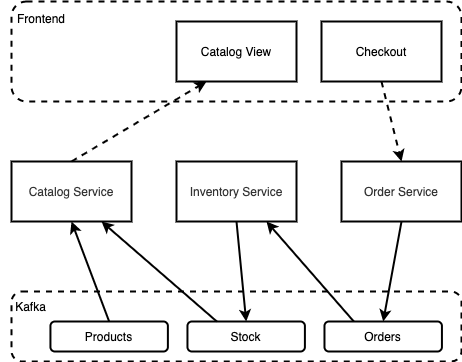
\includegraphics[width=0.8\linewidth]{webshop.drawio.png}
  \caption{Simplified Web-Shop Design Using Apache Kafka}\label{fig:web-shop}
\end{figure}

At the top, the \gls{ui} is comprised of two fragments: the catalog view and the checkout.
The catalog view displays the shop's current inventory to the user, fetching it via a synchronous HTTP request from the catalog service.
At the checkout, the user can order items from the catalog, for which the view sends an HTTP request to the order service.

In the backend, the order service processes users' orders (payments, shipping calculation, \ldots) and publishes \texttt{OrderCreated} events to the \texttt{Orders} topic in Kafka.
% Listing \ref{lst:order-created} shows what the Avro schema for such an event might look like.
Please note, \enquote{event} is a term from \gls{ddd} and describes the record of an occurrence like \enquote{The user created an order.}.
In this example, the microservices communicate by recording and sharing the events occurring in their respective business domain by publishing them as messages to Kafka topics.
Therefore, an event is always a message, but a message is not always an event.

The inventory service consumes the events from the \texttt{Orders} topic and updates the shop's stock accordingly by publishing \texttt{StockUpdated} events to the \texttt{Stock} topic.
These events are read by the catalog service, which also reads from the \texttt{Products} topic.
The service joins these two event streams to materialize a view of the current stock combined with product details, which it presents to the catalog view upon request.

\subsection{Introducing Schemas}

Introducing Avro schemas to the system can make the web-shop more reactive in several ways.
First, if the microservices serialize the contents of their messages using Avro's compact binary format instead of, for example, UTF8-encoded JSON objects, it would reduce the overall size of the messages.
That would increase the system's throughput of messages, potentially making it more responsive.
It also would make more efficient use of the Kafka broker's disk storage.

Furthermore, the introduction of schemas would formalize establishing shared understandings about data between microservices.
Instead of informal communications or semi-formal specifications that development teams exchange, schemas represent formal documents that can be checked for soundness, compared, and managed via version control systems.
This reduces the risk of failures occurring due to \enquote{misunderstandings} and makes the system more resilient.
Additionally, when consumers attempt to de-serialize messages which do not conform to their expected schema, the de-serialization fails.
This fail-early mechanism can prevent more critical failures down the line, thereby contributing to the system's resilience.

Lastly, schema evolution capabilities like Avro's can reduce the coupling between microservices introduced by the need to form a shared understanding about the data they exchange.
Consider this example: The order service makes changes to its data model that also affect the \texttt{OrderCreated} events.
If the order service team deploys the service immediately and it starts publishing messages with the new schema, it would break the communication with the inventory service.
Therefore, both services must start to use the new schema simultaneously.
Without a mechanism like feature toggling, the teams must deploy them simultaneously, which negates one of the main advantages of microservices: That they are independently deployable.
Schema evolution removes the coordination effort for making one-sided, compatible data model changes.
That makes microservices more independent, their development teams more autonomous, and the system more flexible.

\subsubsection{Schema Evolution}

\subsubsection{Schema Revolution}

\section{Schema Management}

\subsection{Schema Management Solutions}

\section{Overview of Schema Management Solutions}
